\documentclass[a4j,11pt]{article}

\usepackage{amsmath,amssymb}
\usepackage{amsthm}
\usepackage{wasysym}


\usepackage{fontspec} %\set~font でフォント設定するにしろ必要
\usepackage{jpnreturn} % 作成したパッケージを読み込む

\setmainfont[ItalicFont=Times Italic]{Hiragino Mincho Pro} %セリフ(ローマン体)のフォント
\setsansfont[ItalicFont=Times Italic]{HiraKakuPro-W3} %サンセリフのフォント ItalicFont でイタリック設定
\setmonofont{HiraKakuPro-W3} %総称ファミリの \ttfamily(等幅,タイプライタ)に割り当てるファミリを指定する

%tikz
\usepackage{graphicx}
\usepackage{tikz}
\usepackage{calc}
\usetikzlibrary{automata,arrows}
\usepackage{array}


\usepackage{wrapfig}
\usepackage{hyperref}


\DeclareMathOperator*{\argmin}{arg\,min}



\title{Oritatami Systemによる\\無限バイナリカウンタの実装}
\author{丸山晃平
\thanks{情報・ネットワーク工学専攻 1831144 関 研究室}
}
\date{令和 2年 1月 20日}%日付


\begin{document}
\maketitle

\section{はじめに}

\section{oritatami system の定義}
$\Sigma$を有限の文字集合とし、その元は塩基の種類を表す。例えば実際のRNAについては$\Sigma = \{ A,U,G,C \}$となる。
$\Sigma^*$と$\Sigma^\omega$はそれぞれ、有限長の塩基配列、無限長の塩基配列を表し、また$\lambda$ は空の塩基配列を表す。
$w = b_1 b_2 \cdots b_n \in \Sigma^*$は長さ$n$の塩基配列を表す。
ここで$n$は正数で、$b_1, \ldots, b_n \in \Sigma$である。
また、$w$の長さは$|w|$で表し、$|w| = n$となる。
$i$、$j$ ($1 \le i \le j \le n$)について、$w[i..j]$は部分配列$b_i b_{i+1} \cdots b_{j-1} b_j$を表し、また$w[i..i]$の場合は単に$w[i]$と表す。


For $k \ge 1$, $w[1..k]$ is called a \textit{prefix} of $w$. 

oritatami system はRNAが転写された際に起こる$cotranscriptional folding$という現象を数理モデル化したものであり、塩基配列$w$を三角格子状の平面グラフ$\mathbb{T} = (V, E)$の上に折りたたまれる。
グラフ上の頂点$p \in V$について、$\hexagon_p^d$は半径$d$、原点$p$の正六角形に含まれる頂点の集合を表す。
なお$\hexagon_p^d$には$3d(d+1)+1$個の頂点が含まれる。
$\mathbb{T}$上の有向パス$P$を$P = p_1 p_2 \cdots p_n$とすると、$p_1, p_2, \ldots, p_n \in V$すなわち、すべての$i $($1 \le i < n$)について$\{p_i, p_{i+1}\} \in E$でありすべての頂点は互いに異なる。
なお、パスの$i$番目の頂点は単に$P[i]$と表す。
今、一本鎖のRNAがoritatami systemに折りたたまれることによってできる「構造」を$C$と定義する。
$C$は$(P, w, H)$の三つの組で表され、それぞれのパラメータについて$P$は$\mathbb{T}$上の有向パス、$w \in \Sigma^*$は$P$と同じ長さの塩基配列、$H$は$H \subseteq \bigl\{\{i, j\} \bigm| 1 \le i, i+2 \le j, \{P[i], P[j]\} \in E \bigr\}$であり、塩基間の水素結合の集合を表す。
なお、$H$についての条件$i+2 \le j$は隣り合う頂点同士が近すぎて物理的に水素結合を結べないという制約を表している。
塩基配列$w$はパス$P$に沿って配置されるため、$w[i]$の配置先は$P[i]$となる。
また、$i$番目の塩基と$j$番目の塩基は水素結合を結ぶことは$\{i, j\}$が$H$に含まれていることと同値である。
構造$C$の長さは塩基配列$w$ともパス$P$とも同じになる。

$R \subseteq \Sigma \times \Sigma$をルールセットと呼び、この$\Sigma$は対称関係になっている。
すなわち、任意の$a, b \in \Sigma$について、$(a, b) \in R$ implies $(b, a) \in R$である。
整数$\alpha \ge 1$は\textit{arity}と呼び、$C$が\textit{arity}$\alpha$であるとき、もしある塩基が$\alpha$の水素結合をしているなら、それ以上その塩基が水素結合をすることはできない。
$\mathcal{C}_{\le \alpha}(\Sigma)$は\textit{arity}が多くとも$\alpha$である$\Sigma$上の構造のことを指し、文脈上で$\Sigma$が明らかな場合は省略して表記する。

\begin{equation}
\label{eq:OS_CF}
C_{i+1} \in \argmin_{
\substack{
C \in \mathcal{C}_{\le \alpha} s.t. \\
C_i \xrightarrow{R}_{w[i+1]}C \\
}
}
\min \Bigl\{ \Delta G(C') \Bigm|
C \xrightarrow{R}^*_{w[i+2...i+k]}C', k\le \delta, C' \in \mathcal{C}_{\le \alpha}
\Bigr\}.
\end{equation}

「周囲の環境」の説明

\section{無限バイナリカウンタの実装}
この章では、oritatami system に実装した無限バイナリカウンタについて説明する。
ここで言う無限バイナリカウンタとは、あるビット幅でカウントアップしていたカウンタが桁上がりのためにオーバーフローした際に、そのビット幅を拡張することでカウントアップを無限に続けていくようなバイナリカウントを指す。


%%%%%%
%% モジュールごとのブリック
%%%%%%
%
% F
%
\begin{figure}[tb]
  \centering
   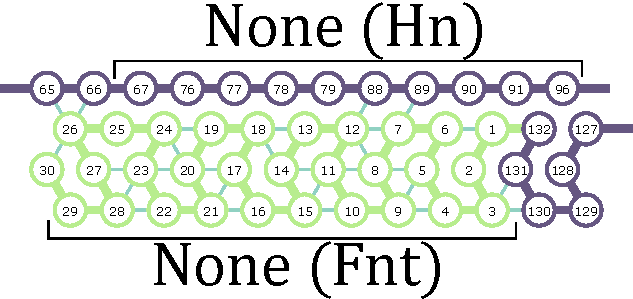
\includegraphics[width=0.6\linewidth]{fig/svg/Fnt_1.pdf}\\
 \vspace*{10mm}
   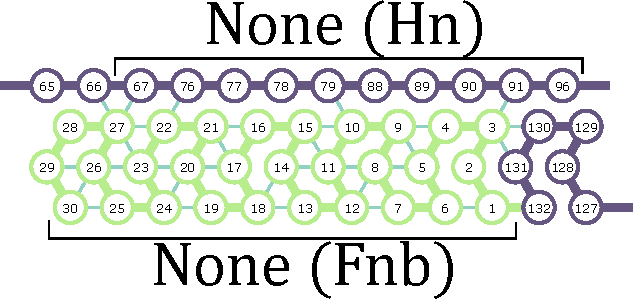
\includegraphics[width=0.6\linewidth]{fig/svg/Fnb_1.pdf}\\
 \vspace*{10mm}
   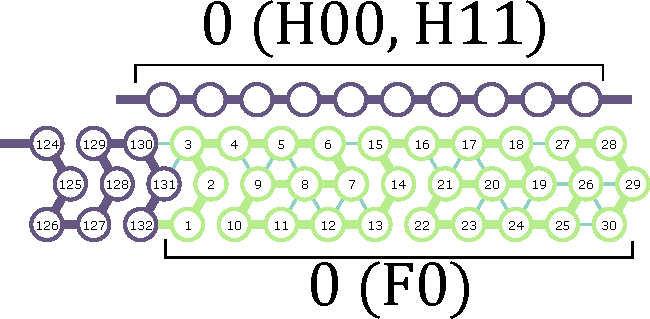
\includegraphics[width=0.6\linewidth]{fig/svg/F0_1.pdf}\\
 \vspace*{10mm}
   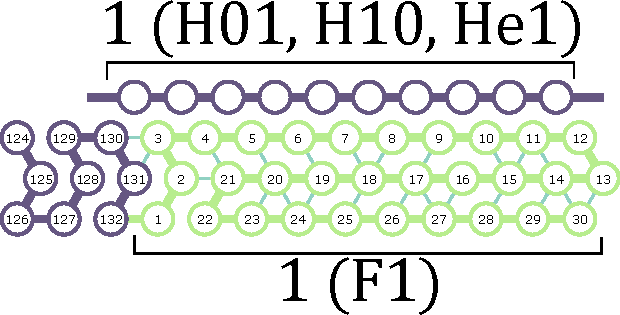
\includegraphics[width=0.6\linewidth]{fig/svg/F1_1.pdf}
 \caption{フォーマットモジュール(F)のブリックは全部で4種類存在する。上二つの\texttt{Fnt}と\texttt{Fnb}はジグでのみ現れ、下二つの\texttt{F0}と\texttt{F1}はザグにのみ現れる。}
 \label{fig:formatters}
\end{figure}

%
% L
%
\begin{figure}[tb]
  \centering
   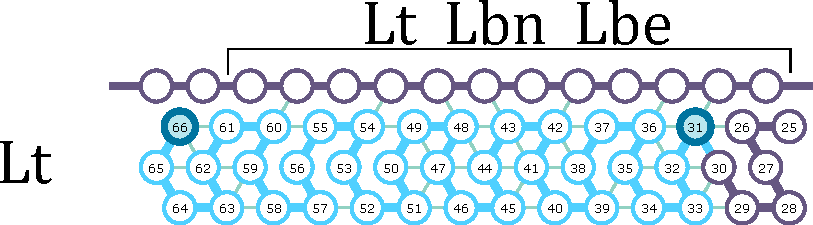
\includegraphics[width=0.6\linewidth]{fig/svg/Lt_3.pdf}\\
   \vspace*{3mm}
   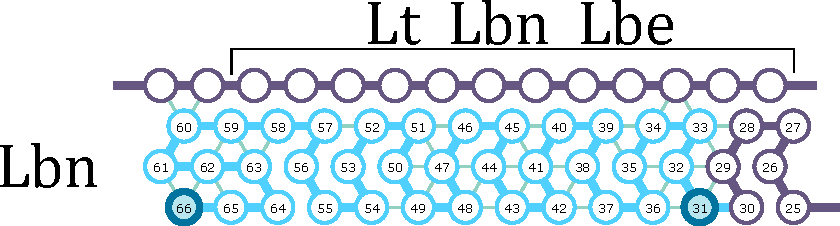
\includegraphics[width=0.6\linewidth]{fig/svg/Lbc_3.pdf}\\
   \vspace*{3mm}
   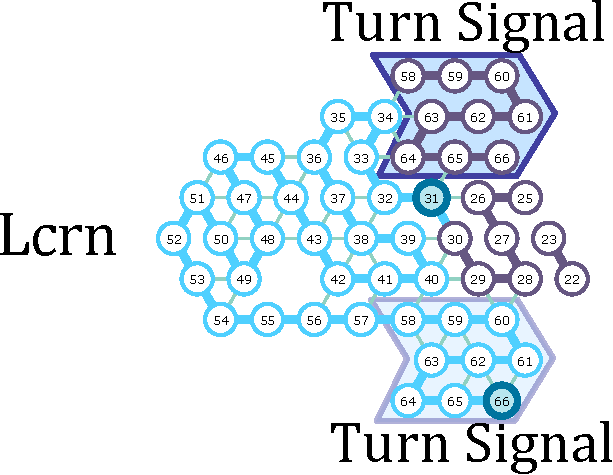
\includegraphics[width=0.4\linewidth]{fig/svg/Ltrc_3.pdf}\\
   \vspace*{3mm}
   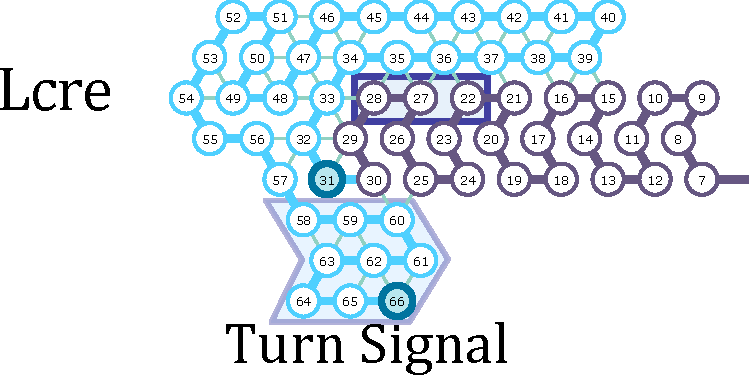
\includegraphics[width=0.5\linewidth]{fig/svg/Ltre_3.pdf}\\
   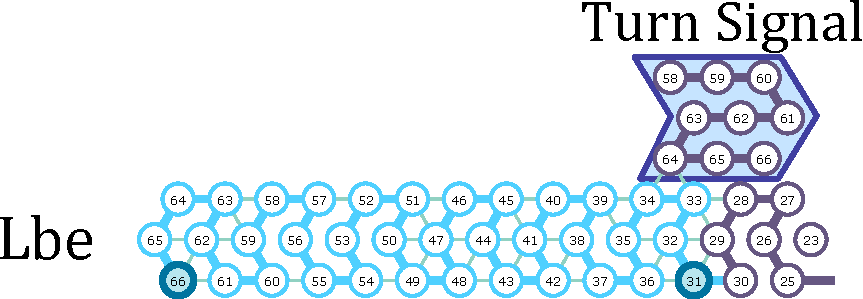
\includegraphics[width=0.6\linewidth]{fig/svg/Lbe_3.pdf}
 
 \caption{左ターンモジュール(L)のブリックは5種類あり、図の上から順に\texttt{Lt}、\texttt{Lbn}、\texttt{Lcrn}、\texttt{Lcre}、\texttt{Lbe}となっている。
ジグの中でLは、左端に到達するまでの間は\texttt{Lt}か\texttt{Lbn}に折りたたまれ、そのどちらになるかはLの折りたたみの開始地点に応じて決定される。
Lが左端に到達した時オーバーフローしていなければ\texttt{Lcrn}、もしオーバーフローしていた時は\texttt{Lbe}に折りたたまれる。
一方でザグの中ではLは\texttt{Lbn}にのみ折りたたまれる。}
 \label{fig:leftturns}
\end{figure}

%
% H
%
\begin{figure}[tb]
  \centering
   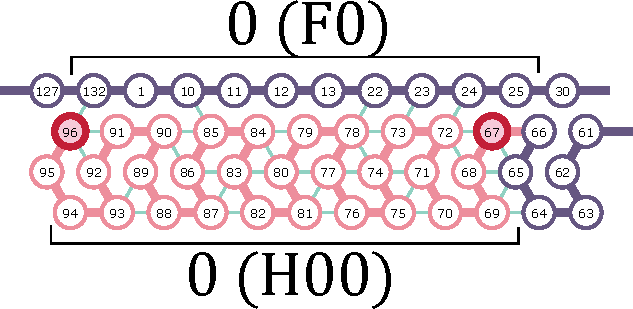
\includegraphics[width=0.45\linewidth]{fig/svg/H00_1.pdf}\\
   \vspace*{3mm}
   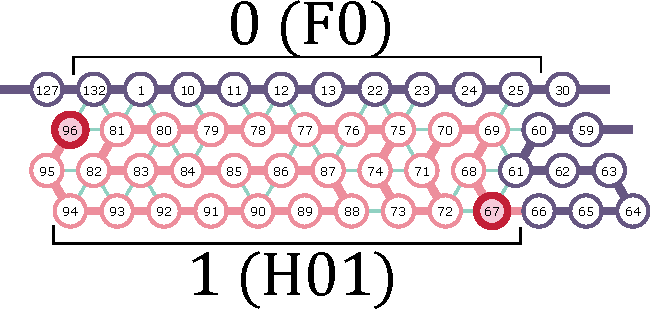
\includegraphics[width=0.45\linewidth]{fig/svg/H01_1.pdf}\\
   \vspace*{3mm}
   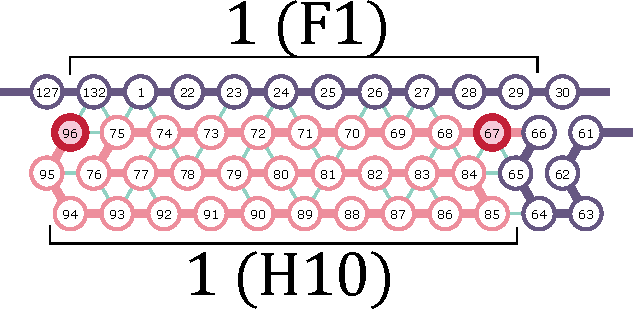
\includegraphics[width=0.45\linewidth]{fig/svg/H10_1.pdf}\\
   \vspace*{3mm}
   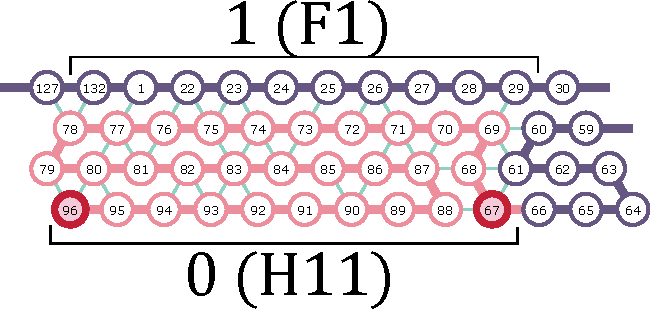
\includegraphics[width=0.45\linewidth]{fig/svg/H11_1.pdf}\\
   \vspace*{3mm}
   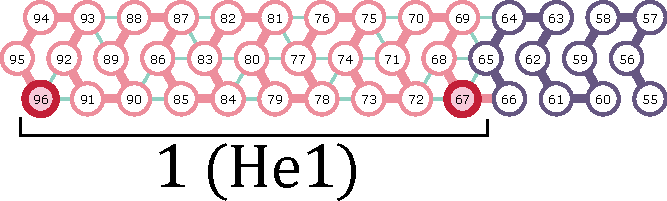
\includegraphics[width=0.45\linewidth]{fig/svg/He1_1.pdf}\\
   \vspace*{3mm}
   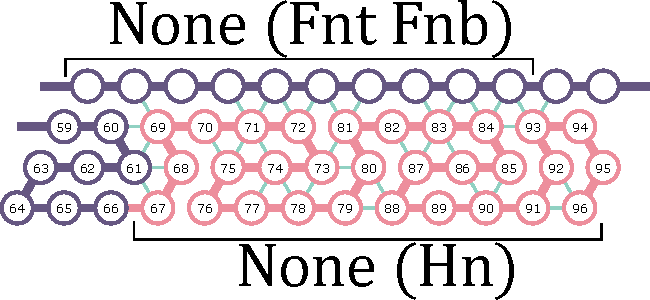
\includegraphics[width=0.45\linewidth]{fig/svg/Hn_1.pdf}

 \caption{半加算器モジュール(H)のブリックは6種類存在し、上から順に\texttt{H00}、\texttt{H01}、\texttt{H11}、\texttt{H10}、\texttt{He1}、\texttt{Hn}となっている。
 ザグの時、Hは\texttt{Hn}にのみ折りたたまれ、ジグの時はそれ以外のブリックに折りたたまれる。}
 \label{fig:halfadders}
\end{figure}

%
% R
%
\begin{figure}[tb]
  \centering
   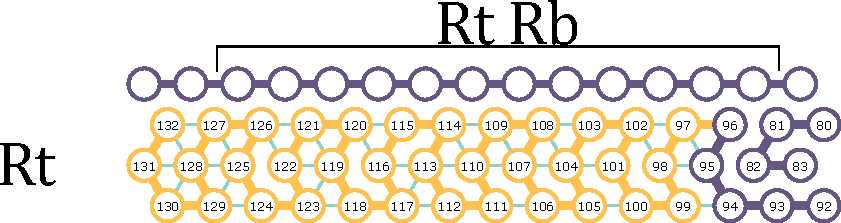
\includegraphics[width=0.8\linewidth]{fig/svg/Rt_1.pdf}\\
   \vspace*{5mm}
   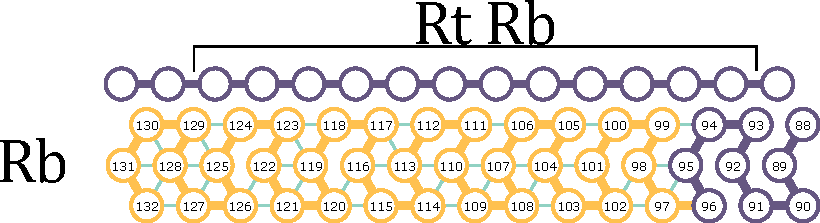
\includegraphics[width=0.8\linewidth]{fig/svg/Rb_2.pdf}\\
   \vspace*{3mm}
   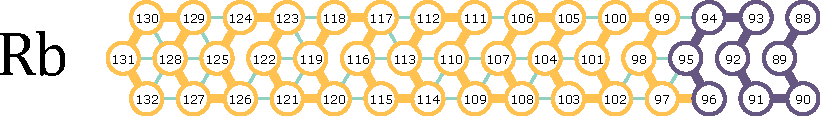
\includegraphics[width=0.8\linewidth]{fig/svg/Rb_1.pdf}\\
   \vspace*{5mm}
   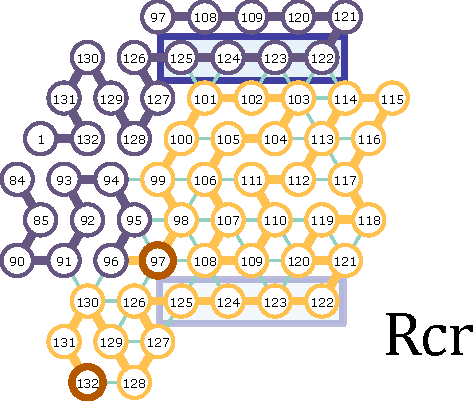
\includegraphics[width=0.5\linewidth]{fig/svg/Rtr_1.pdf}

 \caption{右ターンモジュール(R)は3種類のブリックに折りたたまれる。図は上から順に\texttt{Rt}、\texttt{Rb}(上に構造あり)、\texttt{Rb}(折りたたまれた構造が上に存在しない)、\texttt{Rcr}である。
 ジグの時、Rは\texttt{Rt}か\texttt{Rb}に折りたたまれ、どちらになるかはRの開始地点に依存する。またここでは\texttt{Rb}に関して、2つの内どちらの構造も取り得る。
ザグの時は、右端に到達するまでの間いつもRは\texttt{Rb}(上に構造あり)のブリックに折りたたまれる。
右端にたどり着いたら\texttt{Rcr}へと折りたたまれる。}
 \label{fig:rightturns}
\end{figure}



%%%%%%%%%%
%% brick automaton
%%%%%%%%%%

\begin{figure}[p]
\centering
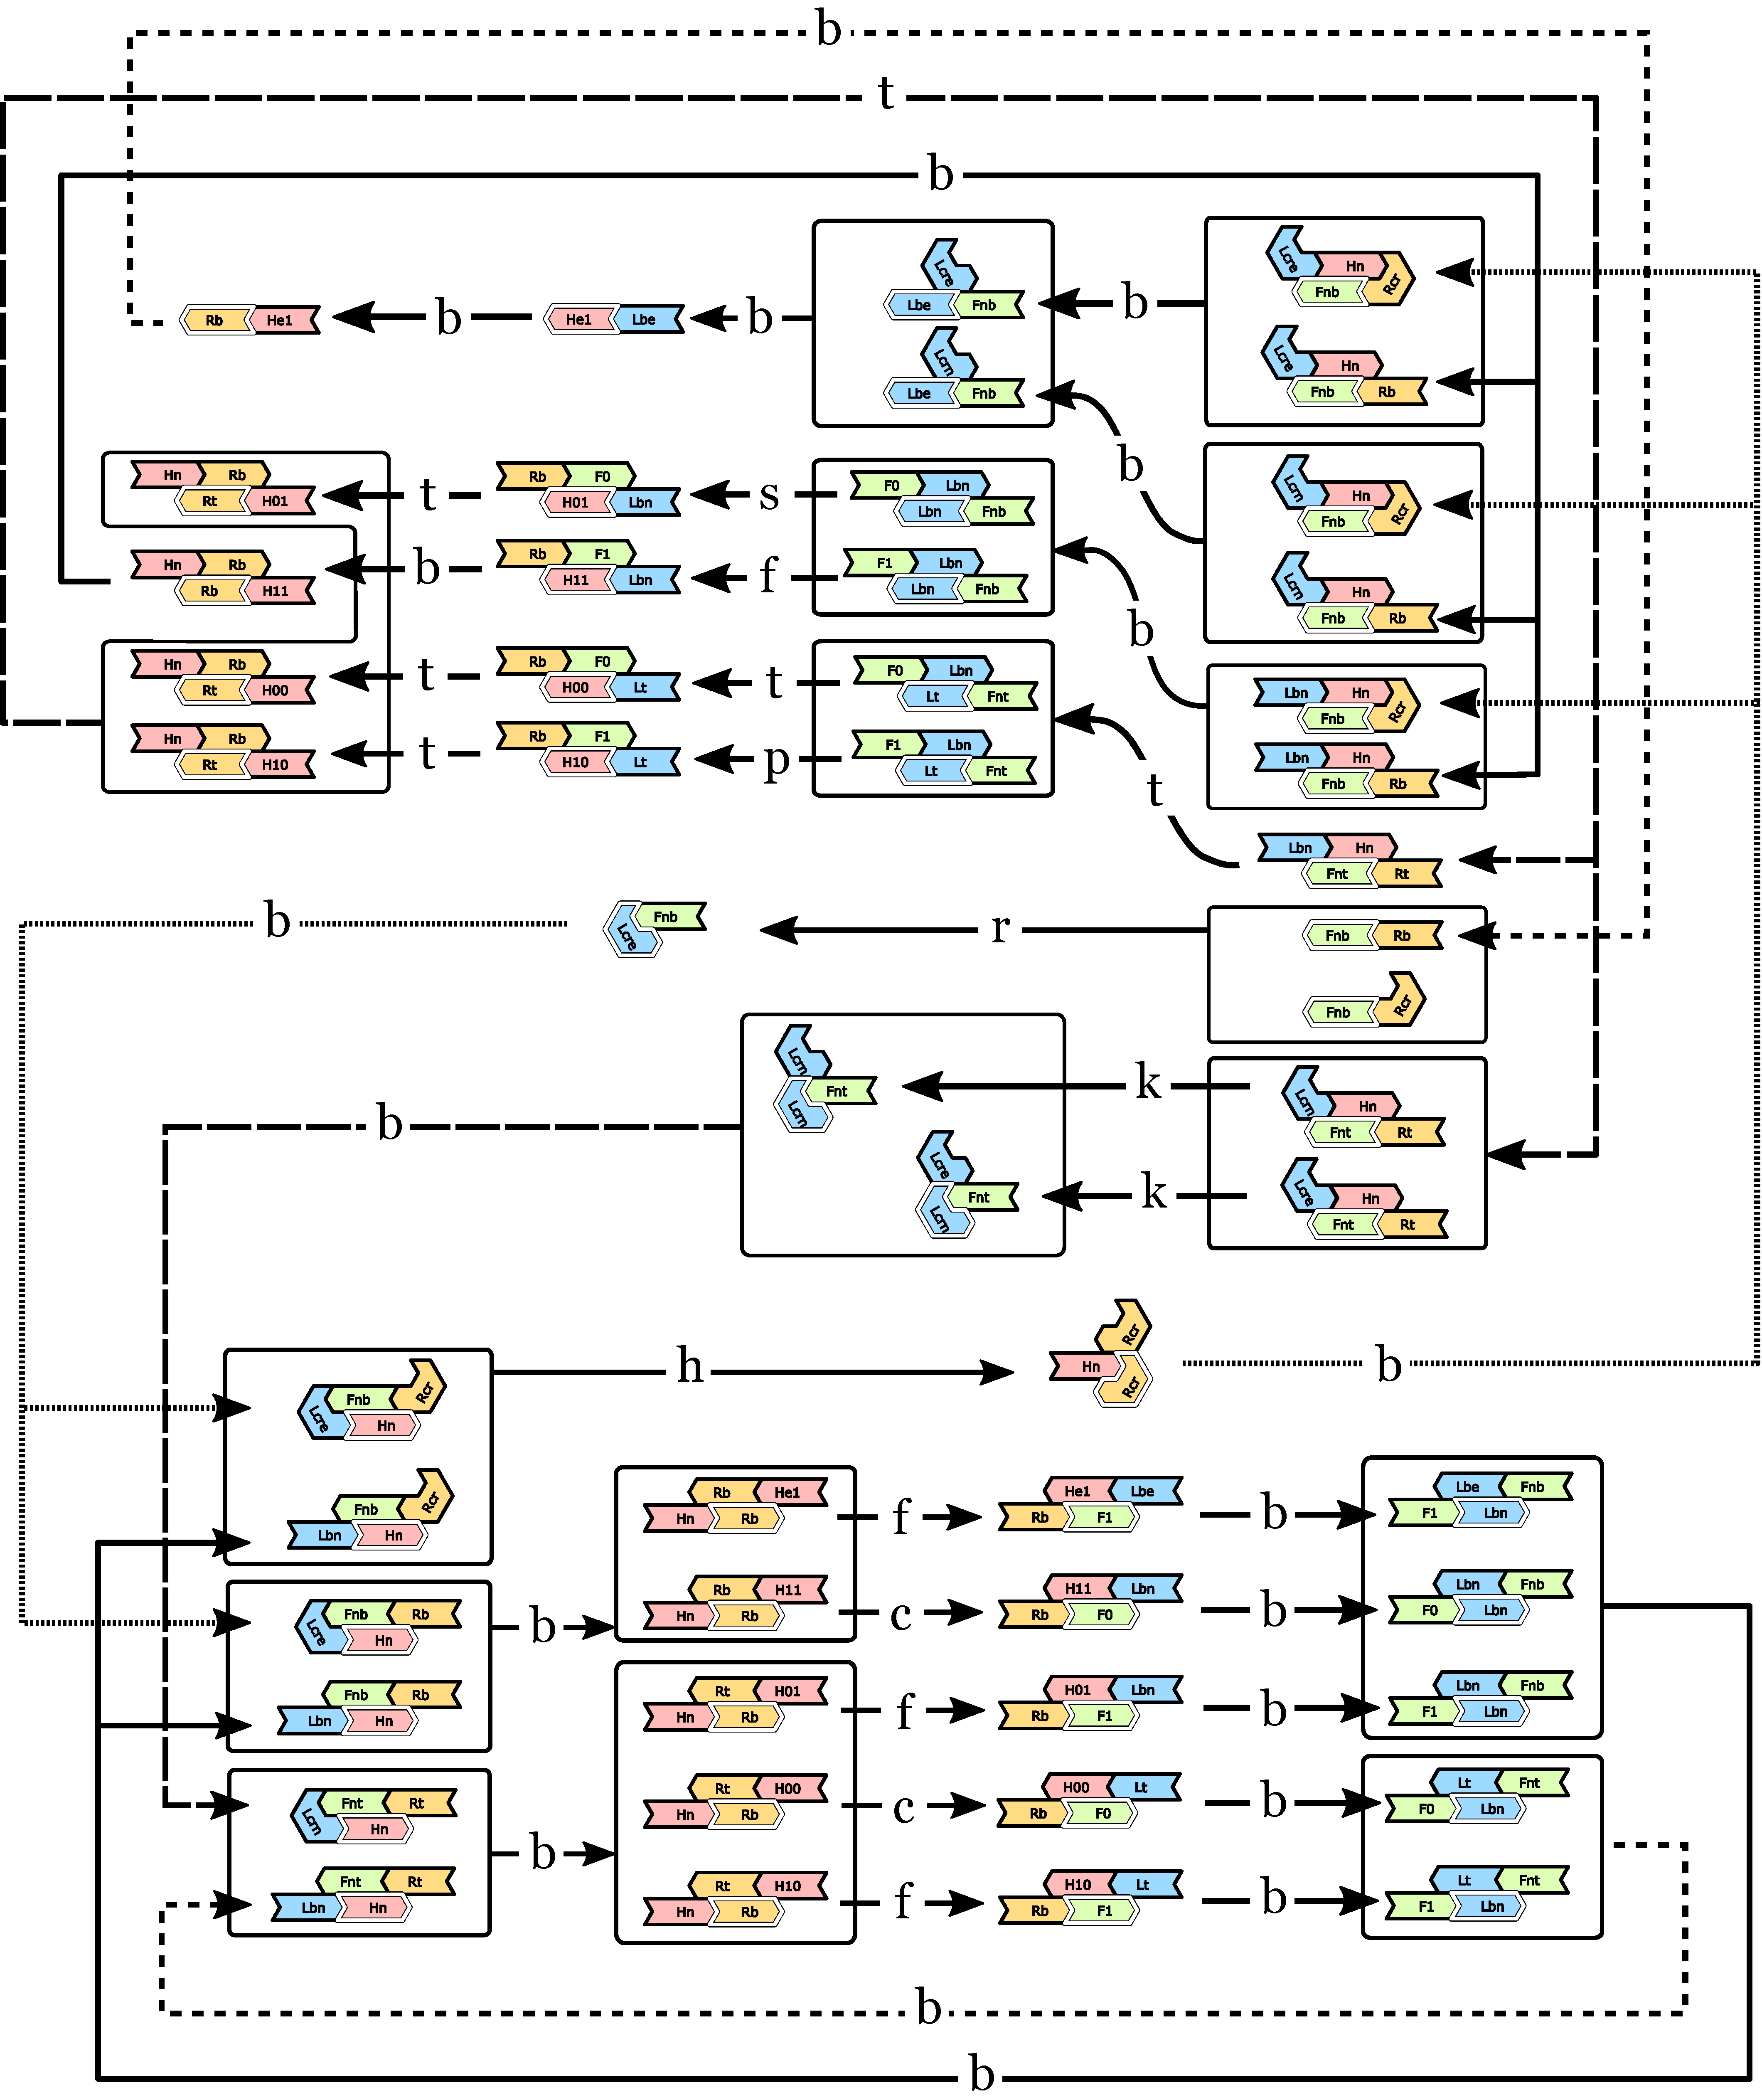
\includegraphics[width=0.95\textwidth]{fig/svg/inf-ai_c_2.pdf}
\vspace*{4mm}

\scalebox{0.68}{
\begin{tikzpicture}
	\node[anchor=north, inner sep=0] (tg) at (0,0) {
 		   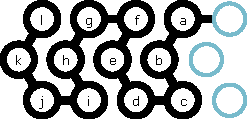
\includegraphics[width=0.2\textwidth]{fig/svg/tglider.pdf}
	};
	\node[anchor=north, inner sep=0] (bg) at (3,0) {
 		   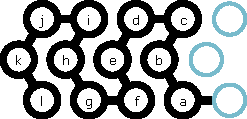
\includegraphics[width=0.2\textwidth]{fig/svg/bglider.pdf}
	};
	\node[anchor=north, inner sep=0] (pl) at (6,0) {
 		   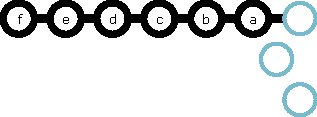
\includegraphics[width=0.2\textwidth]{fig/svg/plane.pdf}
	};
	\node[anchor=north, inner sep=0] (sp) at (9,0) {
 		   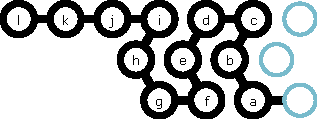
\includegraphics[width=0.2\textwidth]{fig/svg/spiral.pdf}
	};
	
	\node[anchor=north, inner sep=0] (ho) at (-1.5,-3) {
 		   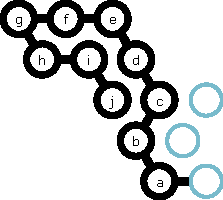
\includegraphics[width=0.2\textwidth]{fig/svg/horn.pdf}
	};
	\node[anchor=north, inner sep=0] (ka) at (1.5,-3) {
 		   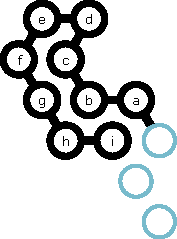
\includegraphics[width=0.15\textwidth]{fig/svg/kar.pdf}
	};
	\node[anchor=north, inner sep=0] (ro) at (4.5,-3) {
 		   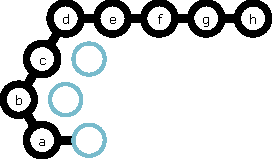
\includegraphics[width=0.2\textwidth]{fig/svg/roof.pdf}
	};
	\node[anchor=north, inner sep=0] (fa) at (7.5,-3) {
 		   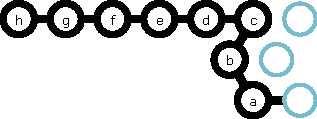
\includegraphics[width=0.2\textwidth]{fig/svg/fault.pdf}
	};
	\node[anchor=north, inner sep=0] (ci) at (10.5,-3) {
 		   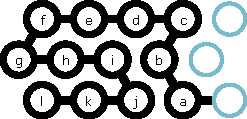
\includegraphics[width=0.2\textwidth]{fig/svg/cliff.pdf}
	};
	
	\node[below, shift=(-90:0.8)] at (tg) {t};
	\node[below, shift=(-90:0.8)] at (bg) {b};
	\node[below, shift=(-90:0.8)] at (pl) {p};
	\node[below, shift=(-90:0.8)] at (sp) {s};

	\node[below, shift=(-90:1)] at (ho) {h};
	\node[below, shift=(-90:1)] at (ka) {k};
	\node[below, shift=(-90:0.8)] at (ro) {r};
	\node[below, shift=(-90:0.8)] at (fa) {f};
	\node[below, shift=(-90:0.8)] at (ci) {c};
\end{tikzpicture}
}
\caption{無限バイナリカウンタのブリックオートマトン}
\label{fig:brickautomaton}
\end{figure}

%%%%%%%
%%%%%%%

\subsection{挙動の概要}
Geary らは有限バイナリカウンタを oritatami system に実装することに成功している\cite{GeMeScSe2019}。
今回実装した無限バイナリカウンタも、基本的な設計方針はこの有限カウンタと同じである。
具体的には、どちらのカウンタの転写物もジグザグ構造に折りたたまれる。
この構造は図において、まずは左方向へ進み、ある段階で折り返して右方向へ進みまた折り返すというように表され、下方向へ段重ねで積み重なっていく。
またジグザク構造のうち、ジグ(右から左への伸長)では現在のカウントが1つカウントアップされ、次のザグ(左から右への伸長)ではジグでカウントアップされた値をフォーマットし、次のジグのためにその値を下方向へコピーするといった挙動も有限カウンタと似ている。
ここで無限カウンタと有限カウンタで異なるのはオーバーフローに遭遇した時の挙動である。
無限カウンタはビット幅を1つ拡張することによってカウントアップを続行する。
%
% 自立したグライダー形にする意義
% グライダーでカウンタを作るには全てを再定義する必要があること
%


実装した無限カウンタの転写物は同じ塩基配列を周期的に繰り返す。
その1周期分の塩基配列は、\texttt{1}-\texttt{2}-\texttt{3}- $\cdots$ -\texttt{132}であり、更にこれは「モジュール」と呼ばれる以下のような4つの部分配列に分けられる。

\begin{itemize}
\item \texttt{1}--\texttt{30}: 「フォーマットモジュール」もしくは「F」と呼ぶ
\item \texttt{31}--\texttt{66}: 「左ターンモジュール」もしくは「L」と呼ぶ
\item \texttt{67}--\texttt{96}: 「半加算器モジュール」もしくは「H」と呼ぶ
\item \texttt{97}--\texttt{132}: 「右ターンモジュール」もしくは「R」と呼ぶ
\end{itemize}

無限カウンタにおける転写物の配列は、この4つのモジュールを用いて$(FLHR)^*$と表すことができる。
また、これらのモジュールは図中ではそれぞれ緑、青、赤、黄色に色分けする。
モジュールはその周囲の環境ごとにそれぞれ特定の平面構造に折りたたまれるように設計されていて、この平面構造のことを「ブリック」と呼ぶ。すなわち、このブリックを「出力」とみなすと、周囲の環境は「入力」であり、oritatami system がモジュールをブリックに折りたたむ過程は情報の「処理」となる。また、出力として扱われたブリックは、別のモジュールにとっての周囲の環境の一部となることによって、情報が伝搬して行く。

例えばフォーマットモジュールについて、そのブリックを見てみる。
フォーマットモジュールは図~\ref{fig:formatters}で示される4種類の環境に遭遇し、それぞれの環境で異なるブリックに折りたたまれる。
これにおいてモジュールがそれぞれのブリックに折りたたまれるのは、式~\eqref{eq:OS_CF}に従って転写配列内の特定の塩基同士が結合するように設計しているためである。

無限カウンタを実装したsystemは、各モジュールが、設計段階で想定された環境にしか遭遇しないことが図~\ref{fig:brickautomaton}の「ブリックオートマトン」によって保証されている。
この遷移図では状態として環境とブリックのペアが、状態間の遷移として、折りたたまれたブリックの前半部分の構造が用いられている。
また、この図で示されているブリックオートマトンは閉じている。
そのため、実装したsystemが正常に動作していることを保証するには、状態ごとの全てにおいて、モジュールが正しいブリックに折りたたまれていることを検証し、かつ遷移先もオートマトンに記述されたものと一致すれば良い。
動作確認は専用に開発したシミュレータに無限カウンタのoritatami systemを適用することで行われ、その結果は\href{https://komaruyama.github.io/oritatami-infinit-counter/}{\texttt{https://komaruyama.github.io/oritatami-infinit-counter/}}に掲載されている。

\subsection{シードへの初期カウント数の記述方法}
初期カウント数がバイナリ表記で$b_{k-1}b_{k-2} \cdots b_1b_0$と表されるとき、シードは以下のように記述される。
\begin{equation} \label{eq:zagencoding}
\texttt{64}{-}\texttt{65}{-}\texttt{66}{-}\left( \prod^0_{i = k-1} \bigl(  w_{Hn} w_{Rb} w_{Fb_i} w_{Lbn} \bigr) \right) w_{Hn}
\end{equation}
ここで、
\begin{eqnarray*}
w_{Hn} &=& \texttt{67}{-}\texttt{76}{-}\texttt{77}{-}\texttt{78}{-}\texttt{79}{-}\texttt{88}{-}\texttt{89}{-}\texttt{90}{-}\texttt{91}{-}\texttt{96},\\
w_{Rb} &=& \texttt{97}{-}\texttt{102}{-}\texttt{103}{-}\texttt{108}{-}\texttt{109}{-}\texttt{114}{-}\texttt{115}{-}\texttt{120}{-}\texttt{121}{-}\texttt{126}{-}\texttt{127}{-}\texttt{132},\\
w_{F0} &=& \texttt{1}{-}\texttt{10}{-}\texttt{11}{-}\texttt{12}{-}\texttt{13}{-}\texttt{22}{-}\texttt{23}{-}\texttt{24}{-}\texttt{25}{-}\texttt{30},\\
w_{F1} &=& \texttt{1}{-}\texttt{22}{-}\texttt{23}{-}\texttt{24}{-}\texttt{25}{-}\texttt{26}{-}\texttt{27}{-}\texttt{28}{-}\texttt{29}{-}\texttt{30},\\
 w_{Lbn} &=& \texttt{31}{-}\texttt{36}{-}\texttt{37}{-}\texttt{42}{-}\texttt{43}{-}\texttt{48}{-}\texttt{49}{-}\texttt{54}{-}\texttt{55}{-}\texttt{64}{-}\texttt{65}{-}\texttt{66}
\end{eqnarray*}
上記の配列は、モジュールH、R、F、Lがブリック\texttt{Hn}、\texttt{Rb}、\texttt{F}$b_i$、\texttt{Lbn}に折りたたまれた時にそのブリックの下部に現れる配列であり、それぞれ図.~\ref{fig:halfadders}、\ref{fig:rightturns}、\ref{fig:formatters}、\ref{fig:leftturns}で確認できる。
例として、初期値$b_0 = 0$、ビット幅$k = 1$のシードは、図~\ref{fig:counter1stzig}における紫色の箇所である。

%%%%
%
%
%
\begin{figure}[p]
\centering
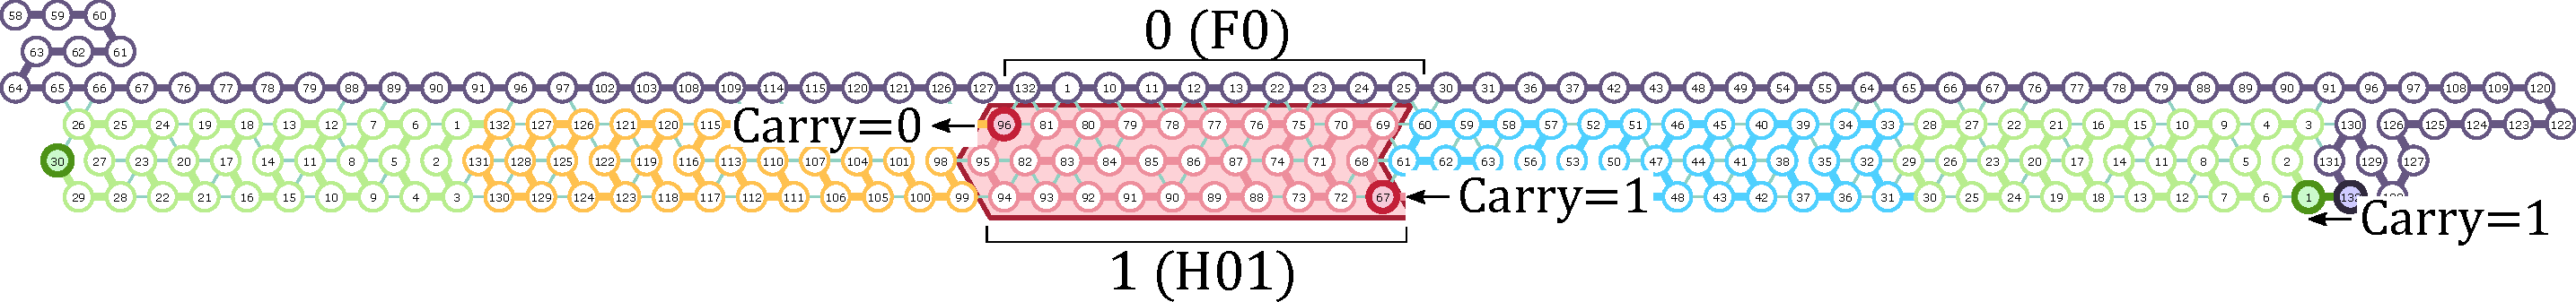
\includegraphics[width=\linewidth]{fig/svg/CounterEx5_1.pdf}
\caption{
一番最初のジグ構造。
\textit{seed}には初期値としての0が式~\eqref{eq:zagencoding}(ビット幅が1すなわち、$k=1$)のフォーマットにしたがって記されている。
また、ジグの始めにキャリーが与えられているので、このジグの中でカウントアップが行われる。
赤色で表された半加算器モジュールHは1を出力し、キャリーを解消している。
またこの1の出力は、正確に言うとザグ内で1と解釈され再フォーマットされるような塩基の並びを指す。
}
%\textcircled{\scriptsize 1}{-}\textcircled{\scriptsize 10}{-}\textcircled{\scriptsize 11}{-}\textcircled{\scriptsize 12}{-}\textcircled{\scriptsize 13}{-}\textcircled{\scriptsize 22}{-}\textcircled{\scriptsize 23}{-}\textcircled{\scriptsize 24}{-}\textcircled{\scriptsize 25}{-}\textcircled{\scriptsize 30},

\label{fig:counter1stzig}
\end{figure}

\begin{figure}[h]
\centering
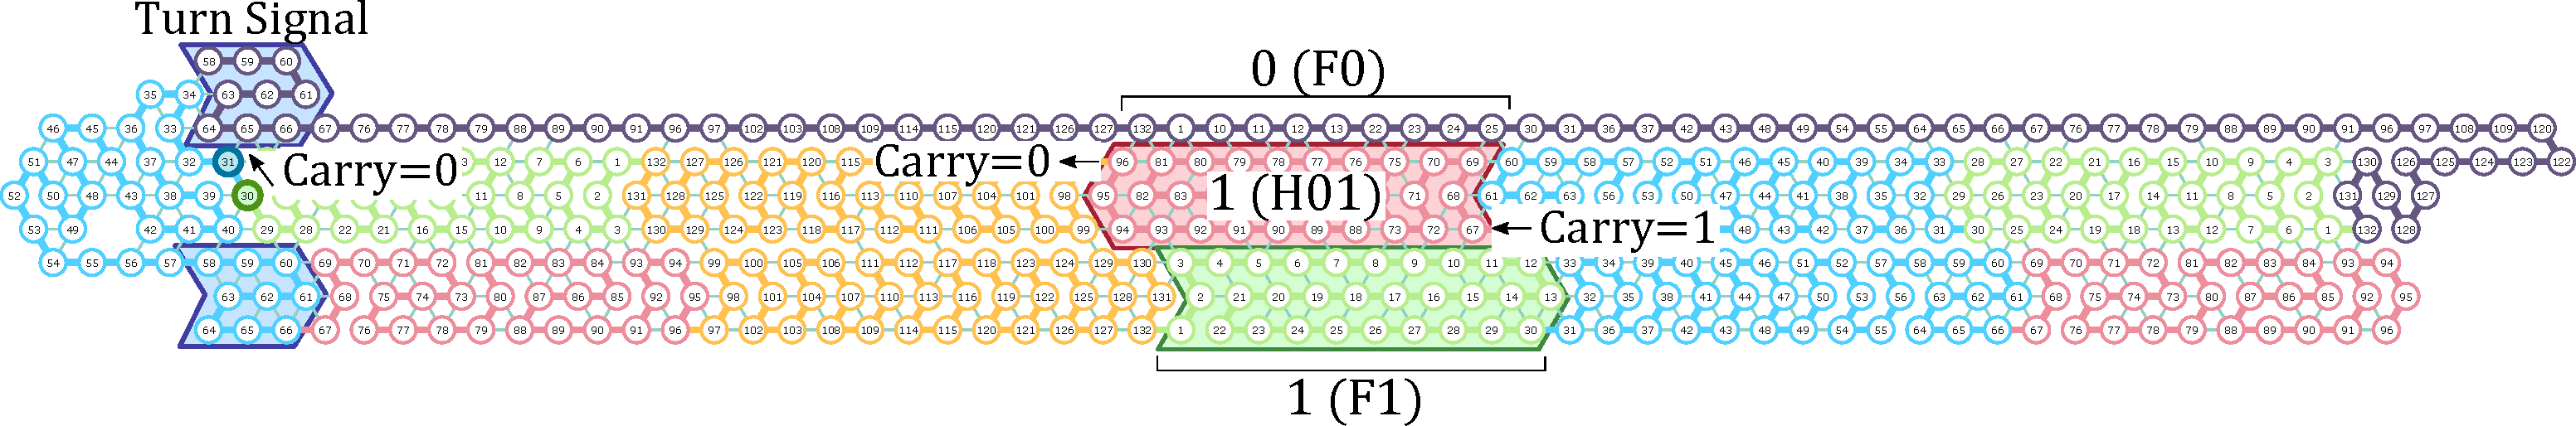
\includegraphics[width=\linewidth]{fig/svg/CounterEx11_1.pdf}
\caption{
モジュールLが左ターンし、最初のジグが始まる様子。
\textit{seed}の左端にターンシグナルがあり、かつジグがキャリーなしで終わっているので、Lはターンシグナルと結合し折り返す。また、ターンしたLのブリックもまたターンシグナルを持つ。
ザグの中ではモジュールFはHの出力を読み、下方向へその値をコピーする。
}
\label{fig:counter1stzag}
\end{figure}

\begin{figure}[h]
\centering
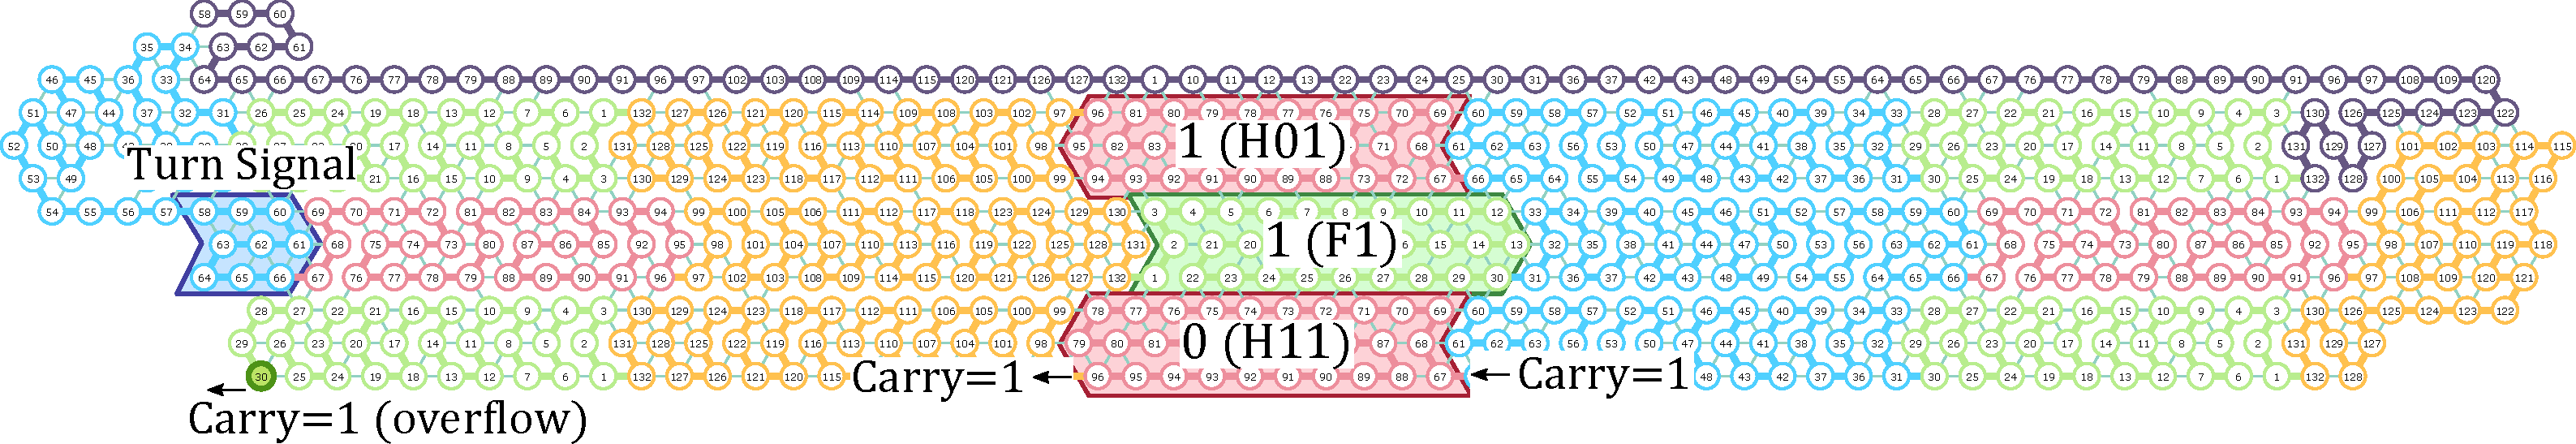
\includegraphics[width=\linewidth]{fig/svg/CounterEx13_1.pdf}
\caption{
キャリーありのまま左端に到達した様子。
この次に転写されるLはジグの下側から転写が開始されるため、上のターンシグナルと結合するには距離が遠すぎる。そのため、Lはターンすることなく直進する。
}
\label{fig:overflowex1}
\end{figure}
%
%
%
%%%%


\subsection{ブリック単位での動作説明}
oritatami systemは最初に\textit{seed}部分が折りたたまれた状態から始まる。
今回実装したsystemでは、ジグ($\leftarrow$)、左ターン($\hookrightarrow$)、ジグ($\rightarrow$)、右ターン($\hookleftarrow$)の4つを周期的に繰り返す。
\textit{seed}に記録された初期カウントが$k$ビットである無限カウンタでは、最初のジグの\textit{transcript}は$(FLHR)^k F$で表される。
ジグの中では、モジュールFとHのブリックはどちらも高さ3、幅10に折りたたまれ、またモジュールLとRのブリックはどちらも高さ3、幅12に折りたたまれる。
それゆえジグは高さ3の線形構造となる。
最初のジグの中で、$i$番目のモジュールHは、式~\ref{eq:zagencoding}に従ってフォーマットされた$b_{i-1}$のすぐ下から転写が開始し、そのフォーマット配列に応じたブリックに折りたたまれる。
つまり、そのHは$b_{i-1}$の値を読んでいることになる。
最初のジグが全て折りたたまれた後、その直後の左ターンモジュールLはターンシグナルのすぐ下に転写される。これによって高さ3のジグがその上側で終了した場合、このターンシグナル(特に\texttt{58}、\texttt{63}、\texttt{64})とLの\texttt{33}と\texttt{34}が結合をし、Lが左ターン用のブリック(\texttt{Lcre})に折りたたまれる(図~\ref{fig:counter1stzag})。
このブリック\texttt{Lcre}は、更に次のジグ終了後にそのブリックの下に転写される左ターンモジュールのためにターンシグナルを持つ。

最初のジグでターンが終わった後に、続いて最初のザグの転写が開始される。
その部分配列は$(HRFL)^k H$で表され、各モジュールについてもジグ同様にモジュールFとHが高さ3、幅10、モジュールLとRが高さ3、幅12のブリックに折りたたまれる。
そのためザグもジグと同様に高さ3の線形構造となる。
このザグが最後まで折りたたまれた直後に転写されるRは、ターンシグナル\texttt{125}-\texttt{124}-\texttt{123}-\texttt{122}と結合することによってブリック\texttt{Rcr}となり右ターンする。
\texttt{Rcr}も次の右ターンのためにターンシグナルを持つ。
このジグとザグが折りたたまれることがカウントの値を一つカウントアップさせることに相当する。

ここで図~\ref{fig:counter1stzig}-\ref{fig:overflowex1}を見てみると、モジュールHとFのブリックが縦方向で交互に並んでいることがわかる。
その列の右から$i$番目がカウンターの$i{-}1$ビットに相当し下方向へカウントの値を伝搬している。


%%
%%
\subsection{カウントアップの方法}
ジグでは、モジュールHが半加算器に相当する役割を果たし、あるHの出力したキャリーは他のモジュール(F、L、R)によって1つ上位ビットのモジュールHへと伝えられる。
無限カウンタ内でキャリーの有無はモジュールそれぞれの転写開始位置によって表現される。
ジグ内で、モジュールF、L、Rはそれぞれ2種類のブリックずつに折りたたまれ、Fは\texttt{Fnt}か\texttt{Fnb}、Lは\texttt{Lt}か\texttt{Lbn}、Rは\texttt{Rt}か\texttt{Rb}になりうる。
これらは図~\ref{fig:formatters}、\ref{fig:leftturns}、\ref{fig:rightturns}を見ると、各モジュールごと一方のブリックが上から転写が始まり上で終わっているならば、もう一方のブリックは下で始まり下で終わっている。
つまり、開始位置(終了位置)が異なる2対のブリックを用いてそれぞれのモジュールはキャリーを伝えている。

ジグは\texttt{Rcr}とシードの開始位置が下側であるのでキャリーが与えられた状態で折りたたみが開始し、カウントアップをしている。
カウントがオーバーフローするまでの間、モジュールHが遭遇し得る環境は、上からの入力が0か1、キャリーが有るか無いかと言う4種類の環境である。
ここで言う上からの入力は、0が$w_{F0}$として、1が$w_{F1}$として表現されている。
そして、この4種類の環境に応じてモジュールHは\texttt{H00}、\texttt{H01}、\texttt{H10}、\texttt{H11}の4つのブリックにそれぞれ折りたたまれる(図~\ref{fig:halfadders})。
なおこのモジュールHについて、ブリックの名称\texttt{H}$xc$は、$x$は入力を、$c$はキャリー(つまり$c=0$ならキャリー無し$c=1$ならキャリー有り)として表している。

図~\ref{fig:counter1stzig}は一番最初のジグが折りたたまれている様子を表している。
ジグは部分配列$(FLHR)^kF$で表され、図中のジグにおいて$k=1$でシードに記述されているカウントの値は$0$である。
ジグは\textit{seed}の終了位置の影響で下側から始まるためキャリーが入力される。
それを、最初に転写されるモジュールFとLがそれに続くモジュールHにまで伝える。
キャリーが入力されたモジュールHは、もしその上に記述された値が$0$であったら図~\ref{fig:counter1stzig}のように\texttt{H01}に折りたたまれ、もし値が$1$なら\texttt{H11}に折りたたまれる。
\texttt{H01}はキャリーを解消するために上側で終了し、一度キャリーが消滅すればそのジグは左端に到達するまでキャリーがない状態が続く。
そしてその状態でジグが終了し次にモジュールLが転写されると、そのLは一つ上のターンシグナルと結合することで通常ターン用のブリック\texttt{Lcrn}に折りたたまれる。
もし、ジグの中で一度もキャリーが解消されない場合、それはすなわちオーバーフローしている場合であり、そのままジグが左端に到達すると次のLは\texttt{Lbe}へと折りたたまれ、オーバーフローの処理に移る。



%%
%%
\subsection{オーバーフローの処理}
Gearyらのカウンターではジグが下側で終了した時、つまりカウントの値がオーバーフローした時にそれを処理できない。
そこで無限カウンタではオーバーフローを処理するために、ジグが下で終わった際にはモジュールLがブリック\texttt{Lbe}に折りたたまれるように設計し、カウントアップの続行を実現した(図~\ref{fig:overflowex2})。
図を見ると、このモジュールLの一つ上にはターンシグナル(\texttt{58}、\texttt{63}、\texttt{64})が存在するが、それがLのターンシグナルである\texttt{33}、\texttt{34}と結合するには遠すぎるので、Lは左ターンしない。
\texttt{Lbe}は自立する構造であるグライダー形であり、周囲に結合を結べるものがなくともそれ自身の内部で結合をすることによって折りたたまれる。
Lに続くモジュールH、R、Fについても何もないところで折りたたみを進行する必要があるため、Lと同様グライダー形となり、それぞれのブリック名は\texttt{He1}、\texttt{Rb}、\texttt{Fnb}である(図~\ref{fig:overflowex3}、\ref{fig:overflowex4})。
なおブリック\texttt{He1}については本質的に\texttt{H00}と同じである。
しかし、この二つは上下が反転していて、このブリックの一段下に来るザグのモジュールから見ると\texttt{He1}は$1$を表す配列が露出していて一方で\texttt{H00}は$0$を表す配列が露出している。

オーバーフローした後に、モジュールL、H、R、Fと転写され、さらにその次に転写されるLを考える。
このモジュールLは、この周囲に何もない空間で左ターンする必要があるが、ターンシグナル存在しなければ再びグライダー形である\texttt{Lbe}となってしまう。
そこで、それを避けるために、Lの\texttt{35}、\texttt{36}が\texttt{Fnb}の上部にある\texttt{28}{-}\texttt{27}{-}\texttt{22}と結合することにする(図~\ref{fig:overflowex4}、\ref{fig:overflowex5})。
つまり、\texttt{Fnb}の左上をターンシグナルとみなすことによってLは左ターン用のブリック\texttt{Lcre}(図~\ref{fig:leftturns})に折りたたまれる。
このためブリック\texttt{Fnb}は常にターンシグナルを持つこととなるが、この左上の箇所は通常(オーバーフローしていない状態)では、一つ上のザグによってターンシグナル部分が隠れているため、必要のない時にモジュールLと結合することを避けることができる。


\subsection{フォーマット}
ジグにおいて半加算器モジュールHが働くことによってカウントアップがされることがわかった。
しかし、カウントの値は式~\eqref{eq:zagencoding}に従ってフォーマットされている必要があり、ジグが終わった段階ではそれは達成されていない。
フォーマットを行うには、モジュールHとFは縦に交互に並んでいることに注目すると、ザグにおいてモジュールHの出力をモジュールFが読み、そして式~\eqref{eq:zagencoding}に従いフォーマットするように設計すれば良い。
すべてのザグはその列の下側から始まる。
これはモジュールLが左ターンする時のブリックは\texttt{Lcrn}もしくは\texttt{Lcre}であり、どちらも下側で終わるためである。
ザグにおいて、モジュール間で横方向には信号を伝える必要がないため、すべてのモジュールはザグの中では下から始まり、下で終わる。
なおかつモジュールH、L、Rについては縦方向にも信号を伝える必要がないため、これらのブリックはそれぞれ\texttt{Hn}、\texttt{Lbn}、\texttt{Rb}にのみ折りたたまれれば十分である。
なおモジュールFについては、Fの一つ上のモジュールHがブリック\texttt{H}$xc$に折りたたまれたのであれば、ブリック\texttt{F}$y$ $(y = (x+c) \mod 2)$ に折りたたまれ、フォーマットを行うように設計した。


%%%%
\subsection{0ビットからのカウントアップ}
有限カウンタでは、1からカウントを始めたとしてもビット幅を定めるために、そのビット幅分の0が記述される。
しかし、この無限カウンタではビット幅が拡張できるため0ビットからのカウントアップすなわち、カウントをの値をシードに記述せずにカウントアップを始めることができる。
シードがカウントの値を持たないのであれば、右ターン用のターンシグナルさえあればいいため%図〜
のようなシードから転写が始まる。
転写が始まると、その上部には折りたたまれた構造が存在しないので、最初のモジュールFからオーバーフローした時と同じ振る舞いをする。
モジュールFはグライダー形に折りたたまり、次のLはFと結合し左ターンする。%図〜
ジグのモジュールFは下側に何も信号を出力しないため、この段階ではまだカウント値は0ビットである。
次にザグに移り、モジュールH、右ターンをするRと続きジグへと移る。
このジグで再びオーバーフローが起こり、ここではカウント値のビット幅が拡張され、値「1」のカウントが行われ、これまで通りのカウントが続く。

\subsection{実装したoritatami system}
今回実装した無限バイナリカウンタのoritatami systemは以下の通りである。
$\Sigma = \{ 1,2, \ldots , 132\}$, $w = p^\omega (p= 1.2.....132)$, $\delta = 3$\\
\raggedright
$R = \{$
(1,6),
(1,74),
(1,75),
(1,77),
(1,80),
(1,81),
(1,84),
(1,93),
(2,21),
(3,130),
(3,131),
(3,64),
(3,65),
(3,84),
(3,91),
(3,93),
(3,95),
(4,21),
(4,83),
(4,84),
(4,9),
(5,20),
(5,8),
(5,85),
(5,9),
(5,90),
(5,91),
(6,15),
(6,19),
(6,81),
(6,82),
(6,83),
(6,84),
(6,91),
(6,92),
(7,12),
(7,13),
(7,18),
(7,83),
(7,89),
(8,11),
(8,12),
(8,18),
(8,73),
(8,78),
(8,87),
(9,17),
(9,72),
(9,73),
(9,83),
(9,86),
(9,87),
(10,15),
(10,67),
(10,79),
(10,81),
(10,85),
(11,14),
(11,15),
(11,64),
(11,66),
(11,78),
(12,33),
(12,61),
(12,63),
(12,64),
(12,65),
(12,66),
(12,77),
(12,78),
(12,81),
(12,88),
(13,18),
(13,30),
(13,31),
(13,32),
(13,33),
(13,72),
(13,81),
(14,18),
(14,29),
(14,30),
(15,28),
(15,39),
(15,72),
(15,76),
(15,81),
(15,90),
(15,91),
(16,21),
(16,27),
(16,38),
(16,39),
(16,71),
(16,72),
(17,20),
(17,21),
(17,26),
(17,27),
(17,70),
(17,88),
(18,25),
(18,27),
(18,67),
(18,69),
(18,70),
(18,71),
(18,72),
(18,88),
(19,24),
(19,26),
(19,71),
(19,81),
(20,23),
(20,24),
(21,37),
(22,27),
(22,28),
(22,36),
(22,75),
(22,76),
(22,78),
(23,26),
(23,27),
(23,28),
(23,73),
(23,74),
(23,75),
(24,71),
(24,72),
(25,30),
(25,60),
(25,69),
(25,73),
(26,29),
(26,30),
(26,31),
(26,65),
(26,66),
(26,69),
(26,70),
(26,71),
(26,72),
(27,35),
(27,36),
(27,64),
(27,66),
(27,67),
(27,68),
(27,69),
(28,33),
(28,35),
(28,60),
(29,31),
(29,32),
(29,33),
(29,40),
(29,60),
(29,69),
(30,32),
(30,33),
(30,39),
(30,40),
(30,60),
(31,36),
(31,65),
(32,35),
(32,36),
(32,37),
(32,38),
(32,56),
(32,57),
(33,35),
(33,47),
(33,48),
(33,61),
(33,63),
(33,64),
(34,39),
(34,45),
(34,46),
(34,47),
(34,58),
(34,63),
(34,64),
(35,39),
(36,43),
(36,44),
(36,45),
(36,60),
(36,64),
(37,42),
(37,43),
(38,41),
(38,42),
(38,43),
(40,45),
(40,58),
(41,43),
(41,44),
(41,45),
(41,57),
(42,54),
(42,56),
(43,48),
(44,47),
(44,48),
(45,51),
(46,51),
(47,49),
(47,50),
(47,51),
(48,50),
(49,53),
(49,54),
(52,57),
(55,60),
(58,63),
(59,62),
(59,63),
(60,66),
(60,69),
(61,66),
(61,67),
(61,68),
(61,69),
(62,65),
(62,66),
(64,69),
(64,85),
(65,67),
(65,68),
(65,69),
(65,84),
(67,131),
(67,72),
(67,84),
(67,88),
(68,72),
(68,83),
(68,84),
(68,87),
(69,130),
(69,131),
(70,75),
(70,81),
(70,87),
(71,74),
(71,75),
(71,81),
(71,86),
(71,87),
(72,79),
(72,80),
(73,78),
(73,80),
(73,81),
(73,84),
(73,88),
(74,77),
(74,78),
(74,83),
(74,84),
(74,87),
(75,132),
(75,83),
(75,96),
(76,81),
(76,87),
(76,93),
(76,95),
(77,80),
(77,81),
(77,86),
(77,87),
(77,92),
(77,93),
(78,127),
(78,132),
(78,99),
(79,84),
(79,88),
(79,90),
(79,96),
(79,97),
(79,98),
(80,83),
(80,84),
(80,88),
(80,89),
(80,95),
(80,96),
(81,132),
(81,89),
(81,96),
(82,87),
(82,93),
(82,94),
(82,95),
(83,86),
(83,87),
(83,92),
(83,93),
(84,131),
(84,93),
(85,130),
(85,90),
(86,90),
(88,93),
(89,93),
(91,130),
(91,96),
(92,96),
(93,130),
(93,132),
(94,99),
(95,97),
(95,98),
(96,130),
(96,132),
(97,102),
(97,108),
(97,126),
(98,102),
(98,106),
(98,107),
(98,108),
(99,106),
(99,127),
(99,129),
(100,105),
(101,104),
(101,124),
(101,125),
(102,123),
(103,108),
(103,113),
(103,114),
(103,122),
(103,123),
(104,107),
(104,108),
(104,113),
(104,115),
(106,111),
(107,109),
(107,110),
(108,124),
(108,125),
(109,114),
(109,120),
(109,123),
(110,113),
(110,114),
(110,119),
(110,120),
(111,117),
(112,117),
(113,116),
(113,117),
(114,122),
(115,120),
(116,120),
(118,121),
(118,123),
(119,121),
(119,122),
(119,123),
(120,123),
(121,126),
(122,126),
(124,129),
(125,127),
(125,128),
(125,129),
(126,129),
(126,130),
(127,129),
(127,132),
(128,130),
(128,131),
(128,132),\}

この無限カウンタは、Gearyらのカウンタと設計の考え方が似ているが、左ターンモジュールにオーバーフローした際の処理と、その後に左ターンしザグに戻る処理を加えることでカウントビット幅の拡張を実現している。
しかし、oritatami systemでは既にGearyらによってチューリングマシンが実装されている\cite{GeMeScSe2018}。
チューリングマシンを用いれば無限カウンタも実装できる。
ただ、このチューリングマシンの使用している塩基の種類数は542種類であるのに対して、今回実装した無限カウンタの塩基の種類数は132であり、より少なくできると言う利点がある。

%%%%
%
%
%
\begin{figure}[p]
\centering
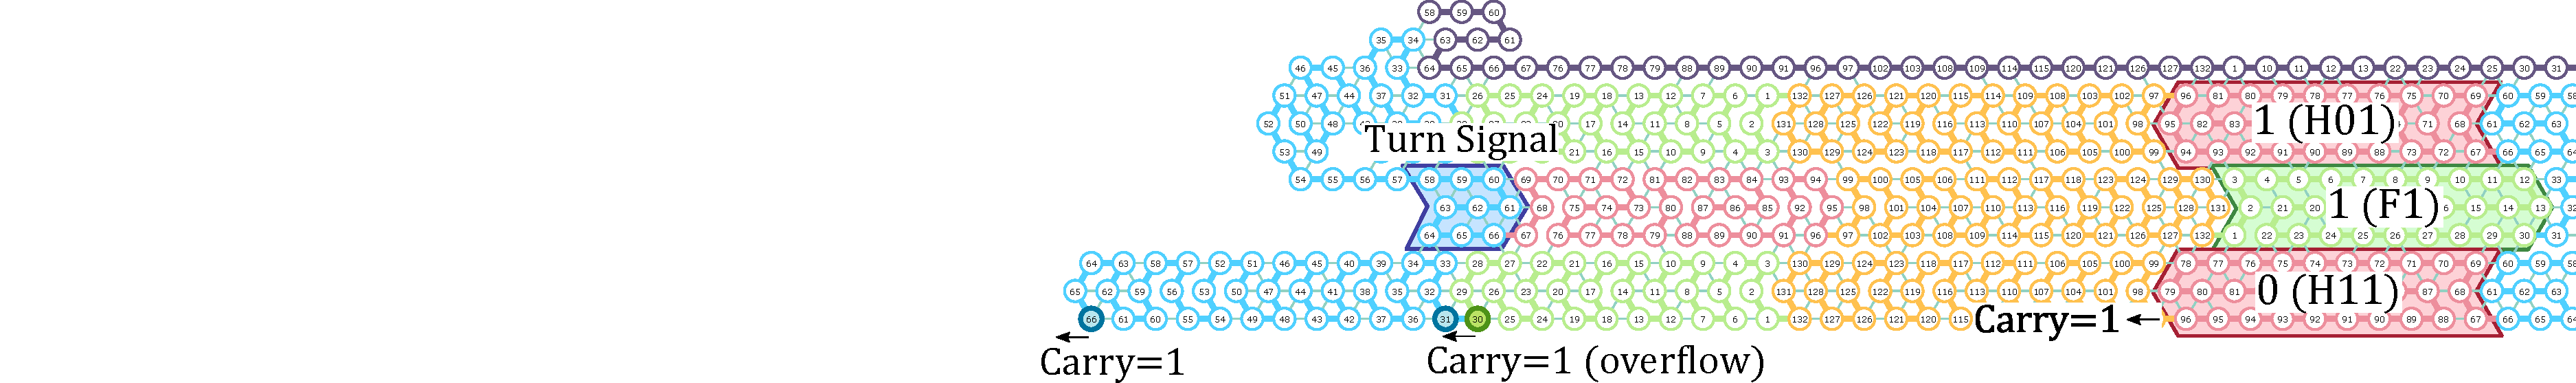
\includegraphics[width=\linewidth]{fig/svg/CounterEx14_1.pdf}
\caption{
モジュールLはターンシグナルと結合せずにグライダー形に折りたたまれ、直進する。
}
\label{fig:overflowex2}
\end{figure}

\begin{figure}[h]
\centering
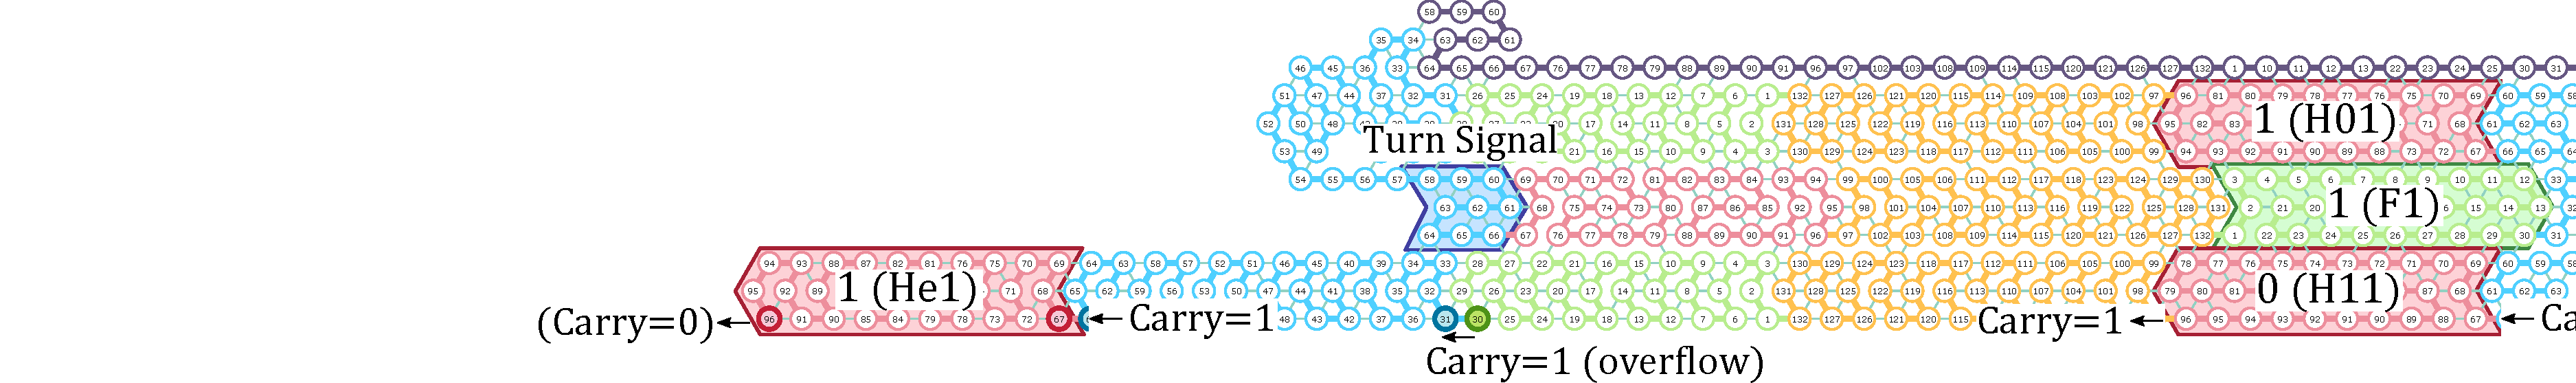
\includegraphics[width=\linewidth]{fig/svg/CounterEx15_1.pdf}
\caption{
モジュールHはオーバーフローのキャリーを受け取るが、H自体は自立できるグライダー形をとる必要があるため、そのキャリーをキャンセルしない。
そのためHの配列の最後は下側に配置されるがキャリーは0として扱われる。
}
\label{fig:overflowex3}
\end{figure}


\begin{figure}[h]
\centering
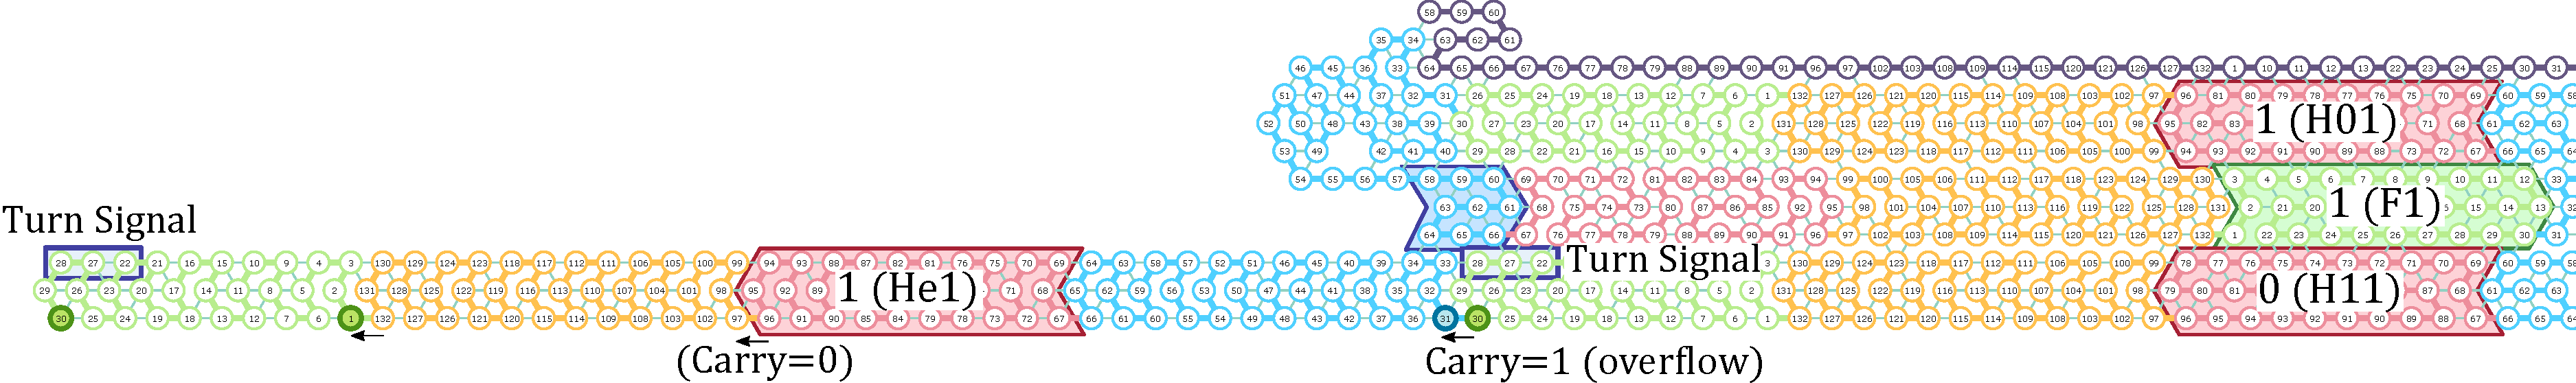
\includegraphics[width=\linewidth]{fig/svg/CounterEx17_1.pdf}
\caption{
モジュールRとFが転写され、続いてモジュールLの折りたたみが開始される。
ここでは、通常のターンのようにターンシグナルを持ったLは周囲に存在しない。
なので、直前のモジュールFの上部をターンシグナルとして扱うことにする。
。
}
\label{fig:overflowex4}
\end{figure}

\begin{figure}[h]
\centering
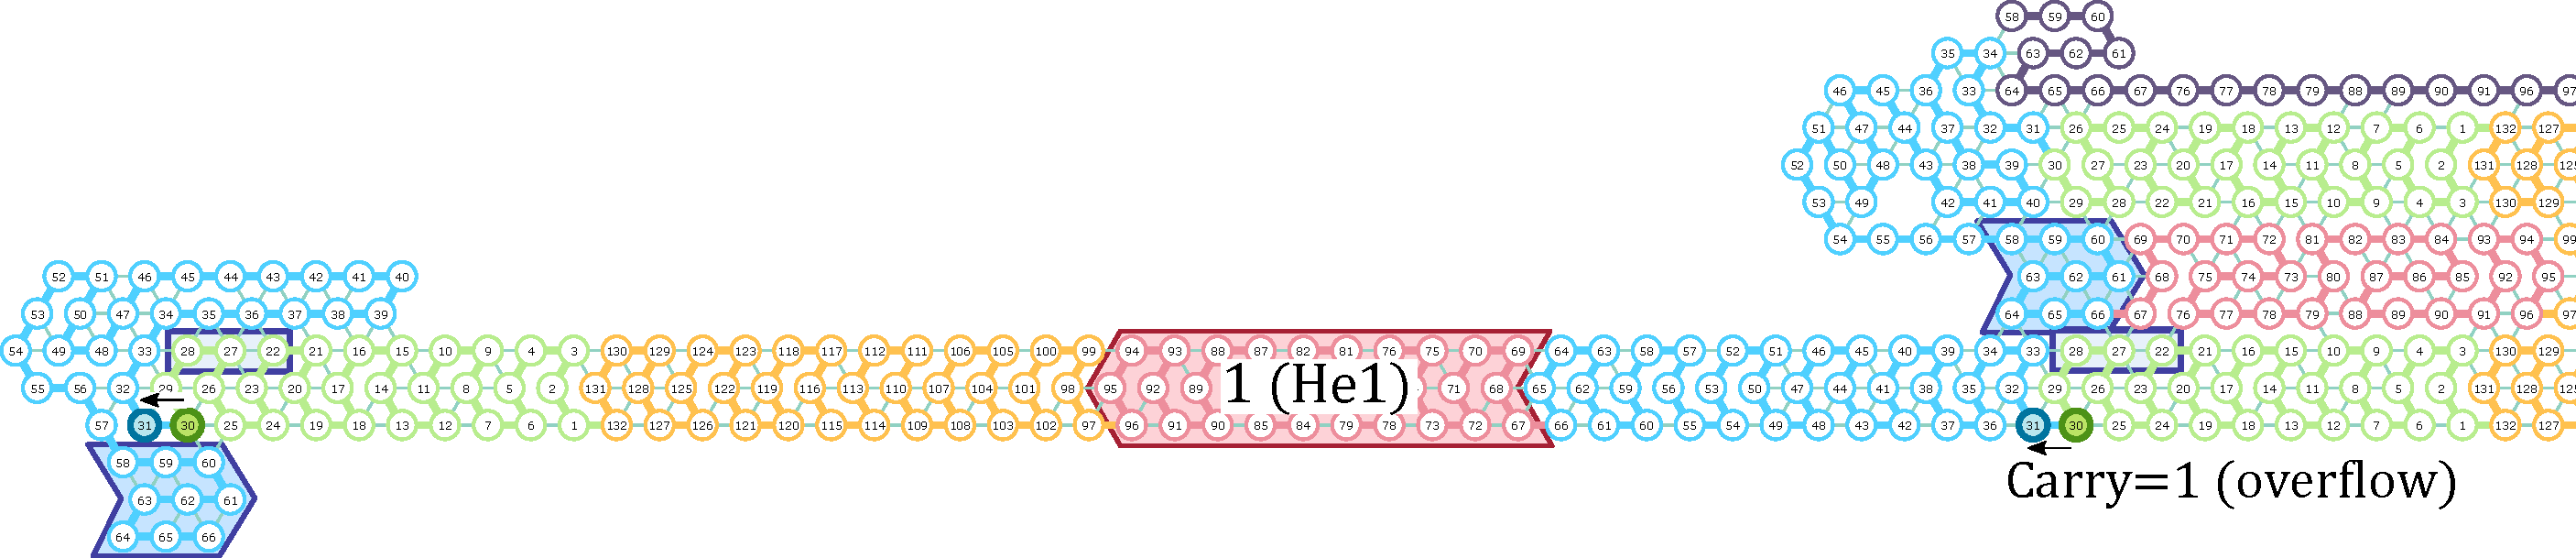
\includegraphics[width=\linewidth]{fig/svg/CounterEx18_1.pdf}
\caption{
モジュールLはFのターンシグナルに結合することによって左ターンし、ザグが開始する。
また、ここで左ターンしたLの最後もターンシグナルとなる。
}
\label{fig:overflowex5}
\end{figure}
%
%
%
%%%%%

\section{$| \Sigma | = 1$における非チューリング完全性について}

\section{まとめ}

\section{謝辞}

\bibliographystyle{plain}
\bibliography{master2020}

\end{document}
